\section{Magnetometr}
Jednym z elementów większości Inercjalnych Systemów Nawigacyjnych jest
magnetometr. Wykorzystuje się go do określenia kierunku w którym porusza się dane
ciało. Typów czujników mierzących pole magnetyczne jest wiele. Dla INS istotny jest jedynie czujnik, będący w stanie wykonać pomiary w zakresie indukcji pola magnetycznego ziemi, która wynosi od $30\mu T$ do $60\mu T$.
\\

\begin{figure}[!ht]
 \centering
 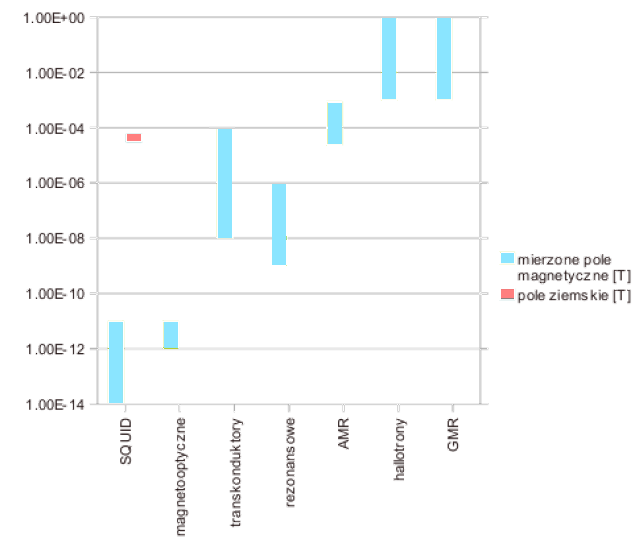
\includegraphics[height=100mm]{../images/ch04/magnetic_sens_types.png}
 \caption{Zakresy czujników pola magnetycznego różnego typu \cite{WstepnyProjektModuluIMU}}
 \label{fig:WykresMagnet}
\end{figure}

Na rysunku \ref{fig:WykresMagnet} przedstawione są zakresy pomiarowe czujników
pola magnetycznego różnego typu. Jak widać tylko dwa rodzaje magnetometrów z
wyżej wymienionych działają w przedziale obejmującym zakres indukcji pola
magnetycznego ziemi. Są to magnetometry transduktorowe oraz AMR\footnote{AMR - Anisotropic Magneto Resistance, anizotropowy magnetoopór}. Z powodu małych rozmiarów, przystępnej ceny i dostępności, w tej pracy wykorzystany został magnetometr AMR.
\\

\subsection{Zasada działania}
Czujnik AMR wykorzystuje zjawisko anizotropowego magnetooporu w celu pomiaru indukcji pola magnetycznego. Zjawisko to objawia się zmianą rezystancji materiału pod wpływem zmiany orientacji działającego pola magnetycznego względem kierunku prądu płynącego przez ten materiał.
\\

Czujniki tego typu charakteryzują się wysoką dokładnością i szybkością działania jednocześnie pobierając mniejszy prąd w stosunku do alternatywnych technologii.

\subsection{Opis elementu}
W celu stworzenia kompasu został wykorzystany magnetometr dwuosiowy MMC2120 firmy Memsic. Dane z magnetometru są przesyłane przy pomocy interfejsu $I^{2}C$ w postaci dwóch 12-bitowych liczb. Jedna z nich określa wartość indukcji pola magnetycznego zmierzonego na osi $X$ druga zaś na osi $Y$. 
\\

\begin{table}[hb]
\rowcolors{2}{white}{gray!20}
\centering
\caption{Parametry magnetometru MMC2120}
   	\begin{tabular}{ | c | c | c | c | p{1.75cm} |} \hline
   		Parametr & Warunki testowe & Wartość & Jednostka \\ \hline
   		Zakres pomiarów & Wypadkowe pole magnetyczne & od $-2$ do $2$ & gauss\\ \hline
   		Nieliniowość & $\pm 1$ gauss & $0.1$ & $\% FS$ \\
   		& $\pm 2$ gauss & $0.5$ & $\% FS$ \\ \hline
   		Dokładność & & od $\pm 2$ do $\pm 5$ & deg \\ \hline
   		Czułość & & od $\frac{1}{461}$ do $\frac{1}{563}$ & gauss \\ \hline
   		Wartość na wyjściu przy & & od $-0.2$ do $0.2$ & gauss \\
   		braku pola magnetycznego & & 2048 & wartość zerowa \\ \hline
   	\end{tabular}
\label{tab:MMC2120Char}
\end{table}

Dla poprawnego działania kompasu niezbędna jest kalibracja magnetometru. Przeprowadzamy ją poprzez obracanie magnetometru we wszystkich możliwych stopniach swobody jednocześnie zapisując wartość maksymalną i minimalną wskazywaną zarówno na osi $X$ jak i $Y$. Dzięki tym wartością będziemy w stanie wyznaczyć, niezależnie dla obydwu osi, przesunięcie wartości zerowej oraz ich czułość.
\textcolor{red}{TODO: WYKRES POMIARU Z NIESKALIBROWANEGO MAGNETOMETRU!}
Kalibrację należy wykonać po umieszczeniu modułu w robocie w celu wyeliminowania zakłóceń spowodowanych metalowymi elementami robota. MMC2120 jako wartość zerową przyjmuje liczbę $2048$. Jest to środek przedziału liczb składającego się z 12 bitów. Wartości poniżej tej liczby są uznawane za ujemne, a wartości powyżej za dodatnie.

\textcolor{red}{TODO: WYKRES POMIARU ZE SKALIBROWANEGO MAGNETOMETRU!}

Niestety z powodu niedokładności samego układu, a także negatywnego wpływu metalowych elementów konstrukcji robota i modułu, wartość zerowa magnetometru może ulec przemieszczeniu. Dlatego też musimy obliczyć odchylenie o jaki należy przesunąć każdy pomiar w celu otrzymania prawidłowego wyniku. Wspomniane odchylenie ten wyznaczamy dla każdej osi jako wartość środkową pomiędzy maksymalnym a minimalnym odczytem podczas kalibracji.

\textcolor{red}{TODO: WYKRES POMIARU ZE SKALIBROWANEGO I NIESKALIBROWANEGO MAGNETOMETRU Z ZAZNACZONYM OFFSETEM!}

Dopiero po właściwym skalibrowaniu magnetometru jesteśmy w stanie wykorzystać go jako kompas. W celu wyznaczenia azymutu, czyli kąta pomiędzy kierunkiem wskazywanym przez oś $X$, \textcolor{red}{TODO: SPRAWDZIĆ KTÓRĄ OŚ FAKTYCZNIE!} a kierunkiem północnym, należy skorzystać z prostego wyrażenia trygonometrycznego przedstawionego na wzorze \ref{eq:azymut}.

\begin{equation}
  \label{eq:azymut}
  \alpha = arctg \left( \frac{y}{x} \right)
\end{equation}

Podczas odczytu wskazań kompasu istotne jest także wzięcie pod uwagę takich czynników jak odchylenie osi $X$ i $Y$ czujnika od kierunku równoległego do kierunku pola magnetycznego ziemi.
\textcolor{red}{TODO: WYKRES POMIARU ZE SKALIBROWANEGO MAGNETOMETRU ALE NIERÓWNOLEGLE DO POLA!}

\subsection{Budowa modułu}
Płytka modułu kompasu została zaprojektowana przy pomocy darmowej wersji programu Eagle na podstawie danych zawartych w nocie katalogowej czujnika MMC2120. Na rysunkach \ref{fig:MMC2120Pcb} oraz \ref{fig:MMC2120Sch} przedstawiono schemat oraz layout płytki modułu kompasu.

\begin{figure}[!ht]
 \centering
 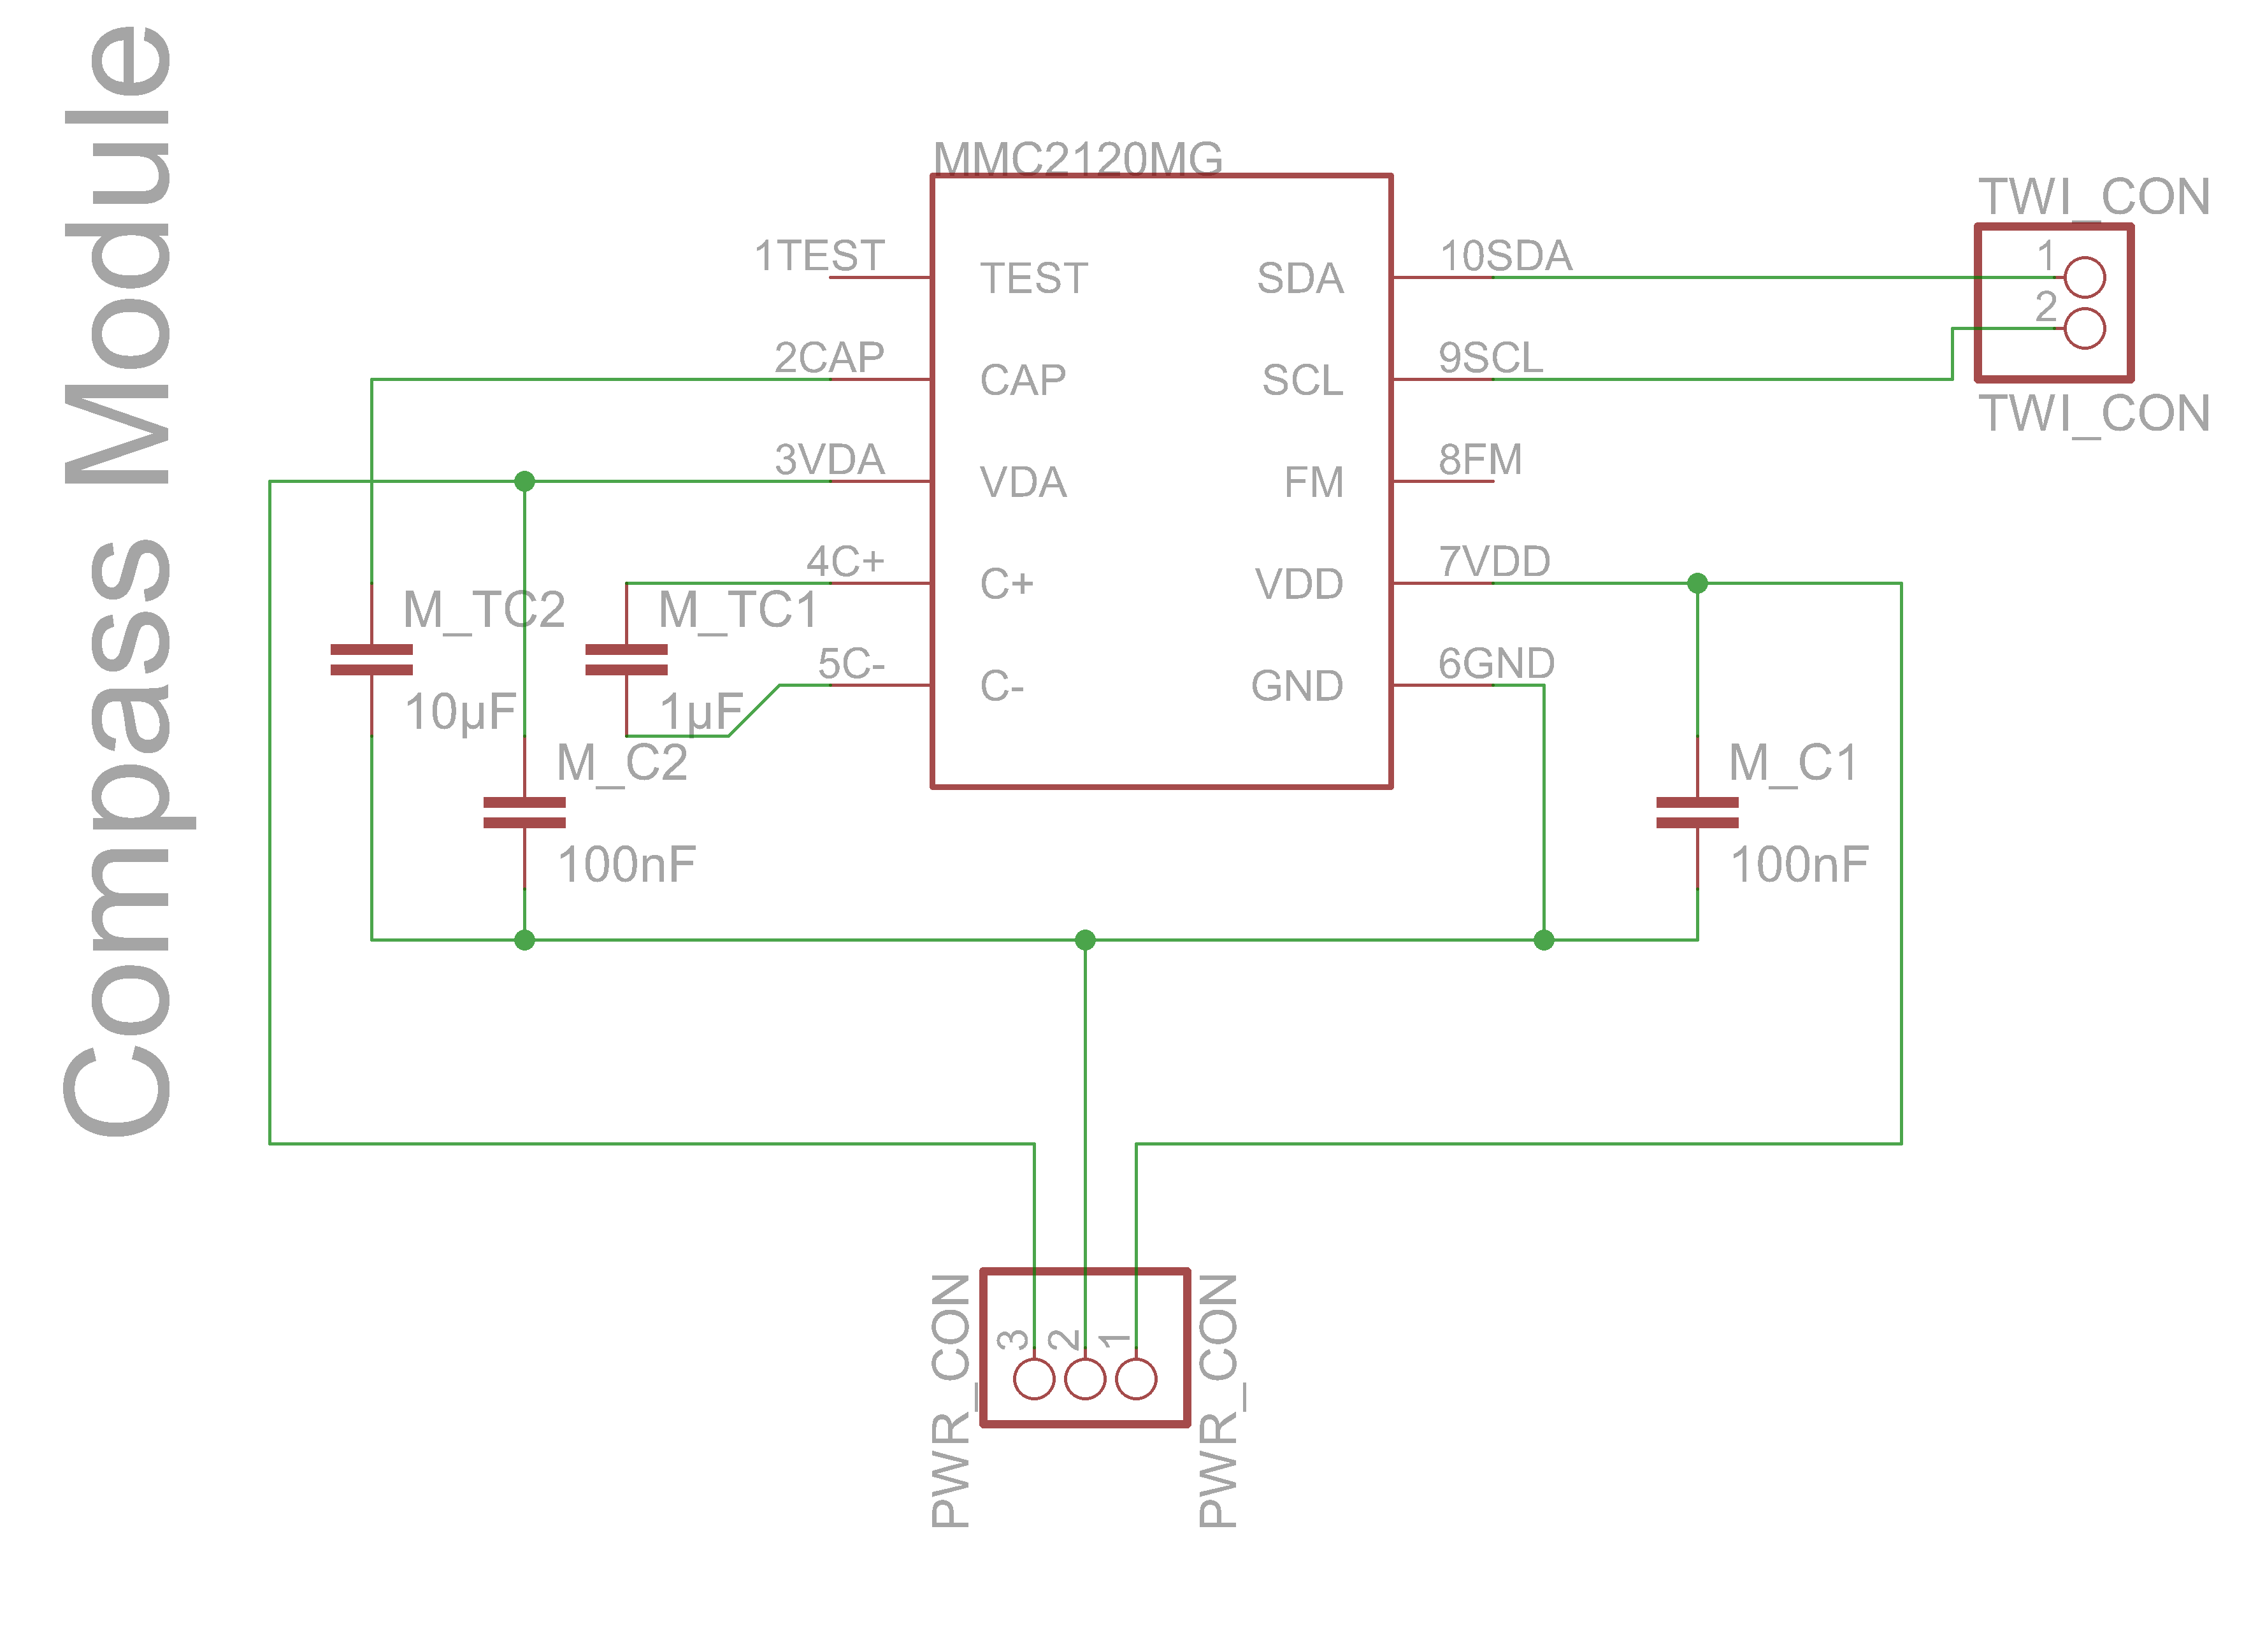
\includegraphics[height=75mm]{../images/ch04/mmc2120mgsch.png}
 \caption{Schemat modułu kompasu}
 \label{fig:MMC2120Sch}
\end{figure}

\begin{figure}[!ht]
 \centering
 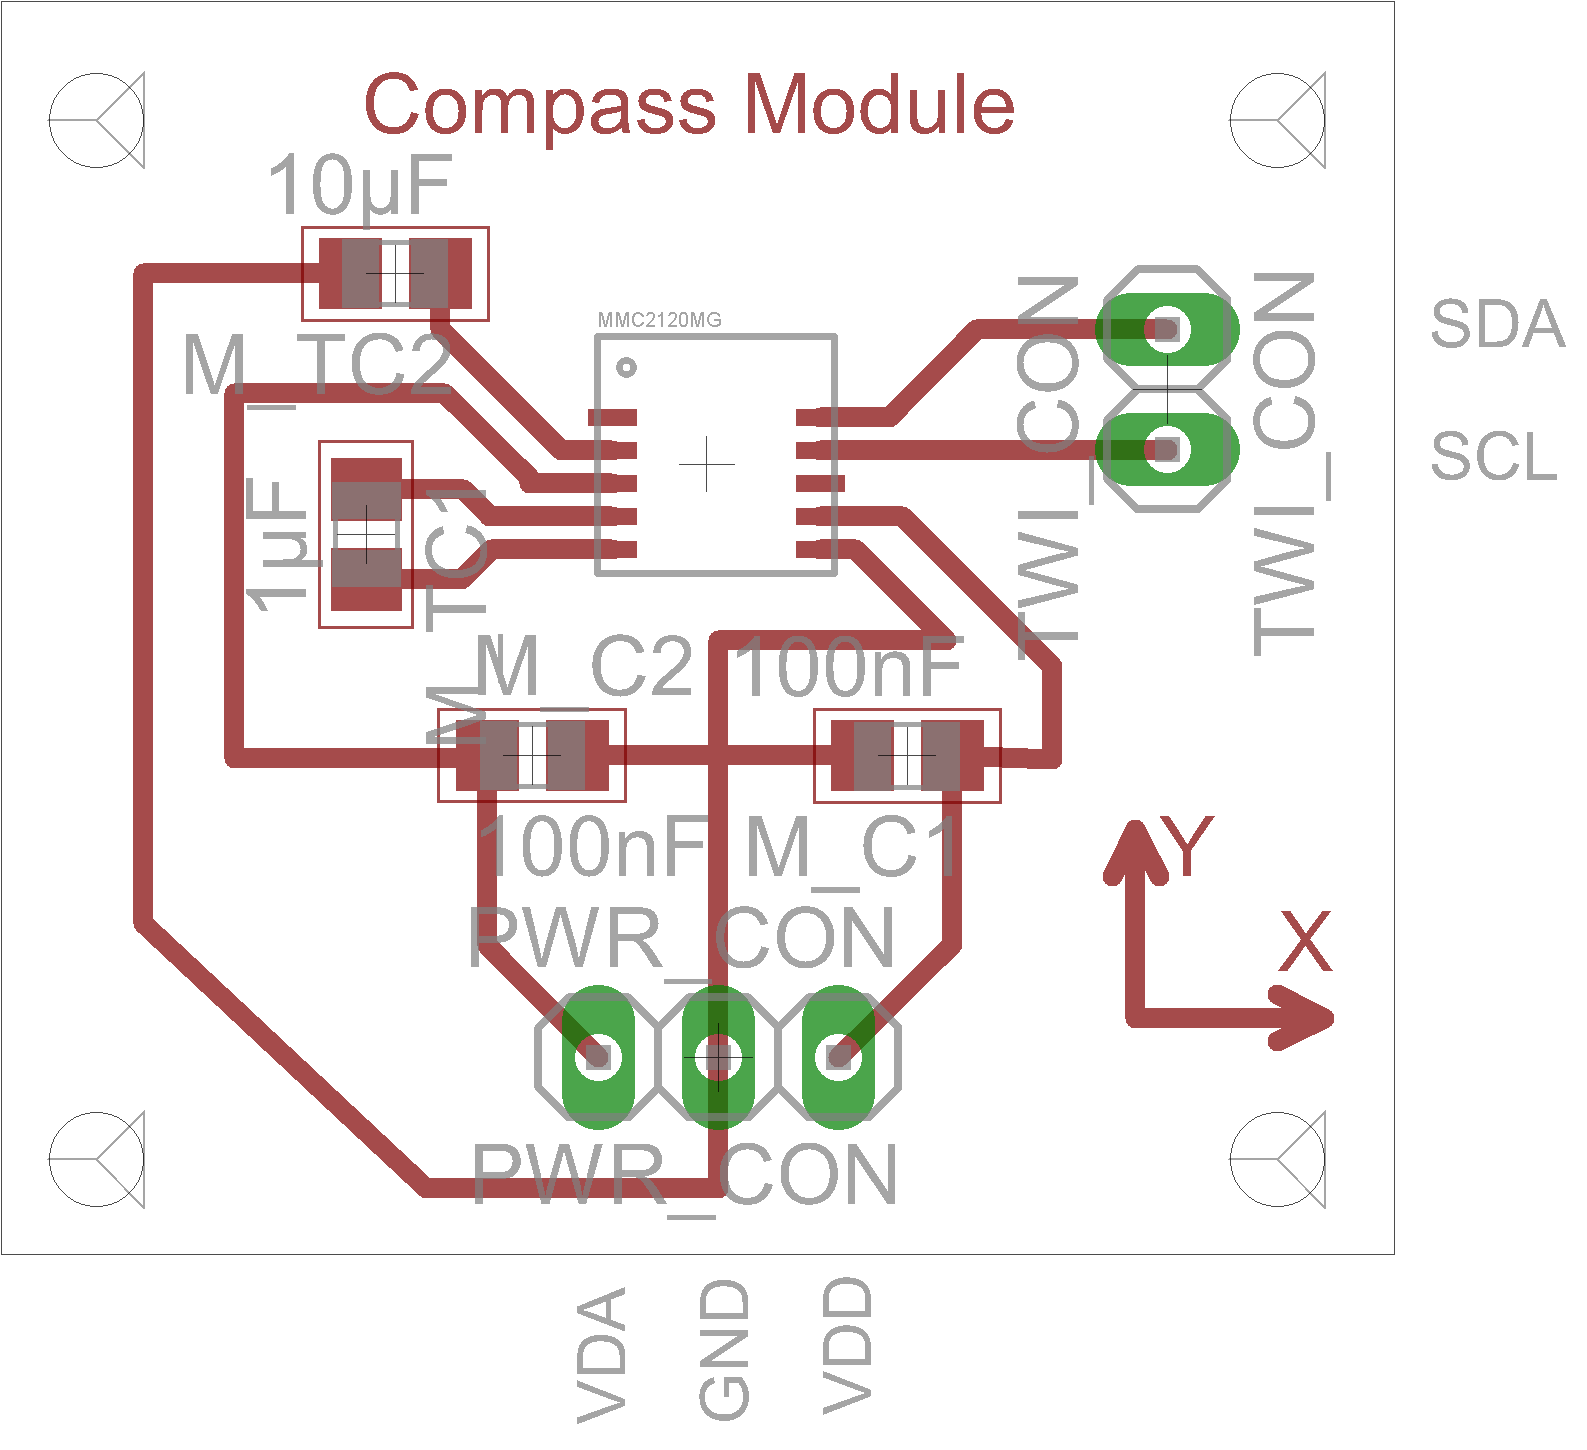
\includegraphics[height=50mm]{../images/ch04/mmc2120mgpcb.png}
 \caption{Projekt płytki kompasu elektronicznego}
 \label{fig:MMC2120Pcb}
\end{figure}

\begin{table}[hb]
  \rowcolors{2}{white}{gray!20}
  \centering
  \caption{Opis wyprowadzeń modułu kompasu}
  \begin{tabular}{ | c | c | c | p{1.75cm} |} \hline
    Nazwa & Typ & Opis \\ \hline
    VDA & Zasilanie & Napięcie zasilania $3.3V$ \\
    GND & Zasilanie & Masa \\
    SCL & Wejście & Zegar sterujący $I^{2}C$ \\
    SDA & We / Wy & Szyna do przesyłania danych $I^{2}C$ \\
    VDD & Zasilanie & Napięcie zasilania szyny danych $3.3V$ \\ \hline
  \end{tabular}
  \label{tab:MMC2120ModOut}
\end{table}

\begin{figure}[!ht]
 \centering
 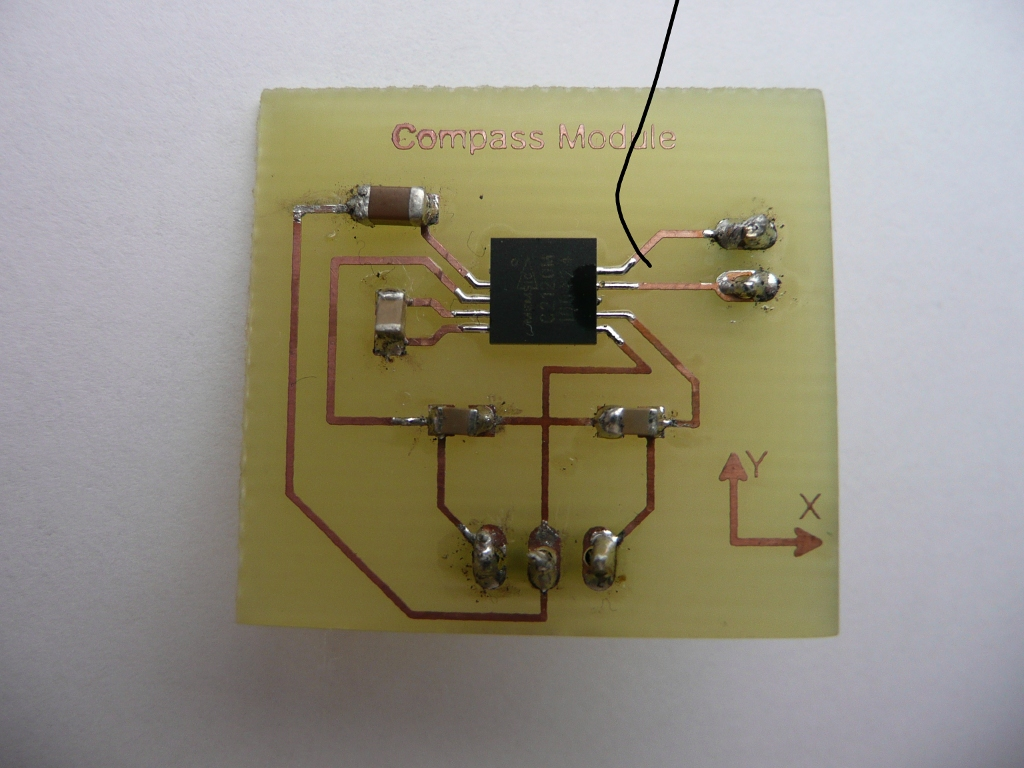
\includegraphics[height=50mm]{../images/ch04/compassmodule.jpg}
 \caption{Gotowy moduł kompasu}
 \label{fig:MMC2120Module}
\end{figure}

\subsection{Nieudana próba zastosowania}
Docelowo moduł kompasu miał być wykorzystywany jako element Inercjalnego Systemu Nawigacji w celu określania kierunku w którym robot się przemieszcza. Zasada działania miała być prosta. Robot miał zapamiętywać aktualny azymut z jakim się poruszał będąc na rekach operatora. Następnie po postawieniu na podłożu miał odtwarzać tor ruchu obracając wszystkie zapamiętane azymuty o $180\circ$. 

\begin{figure}[!ht]
 \centering
 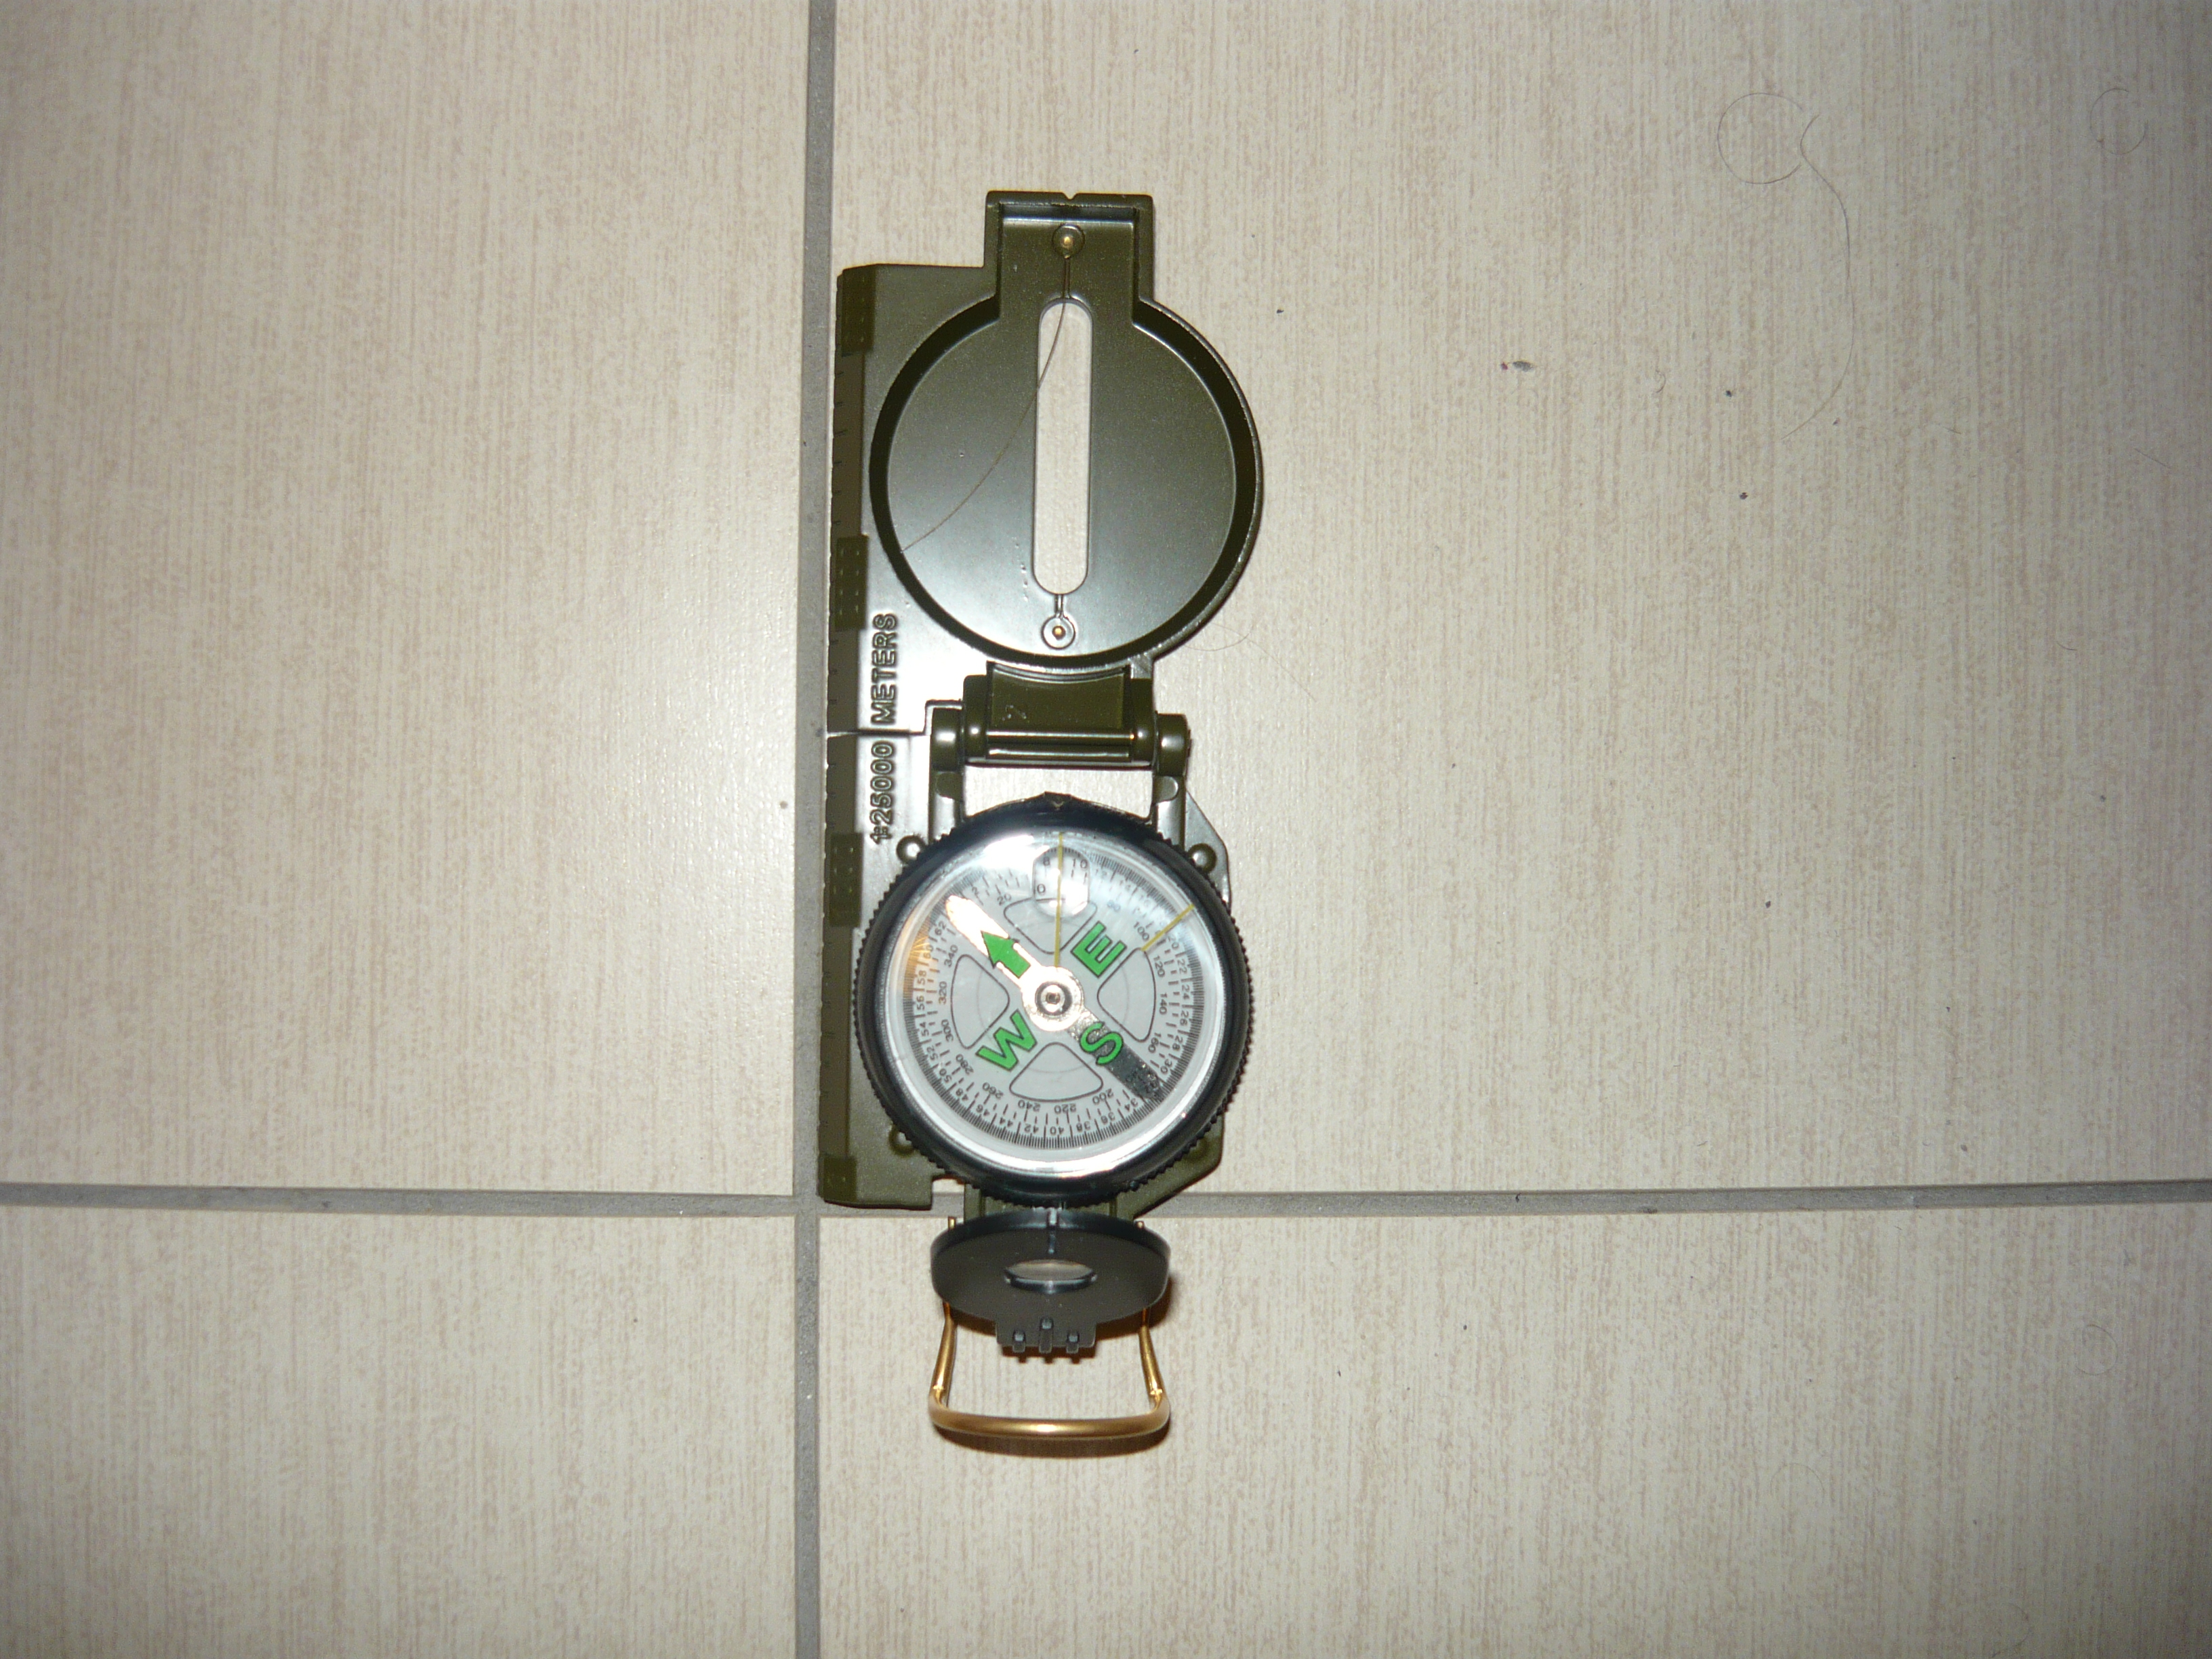
\includegraphics[height=60mm]{../images/ch04/compass01.jpg}
 \caption{Busola w położeniu początkowym}
 \label{fig:Busola1}
\end{figure}

\begin{figure}[!ht]
 \centering
 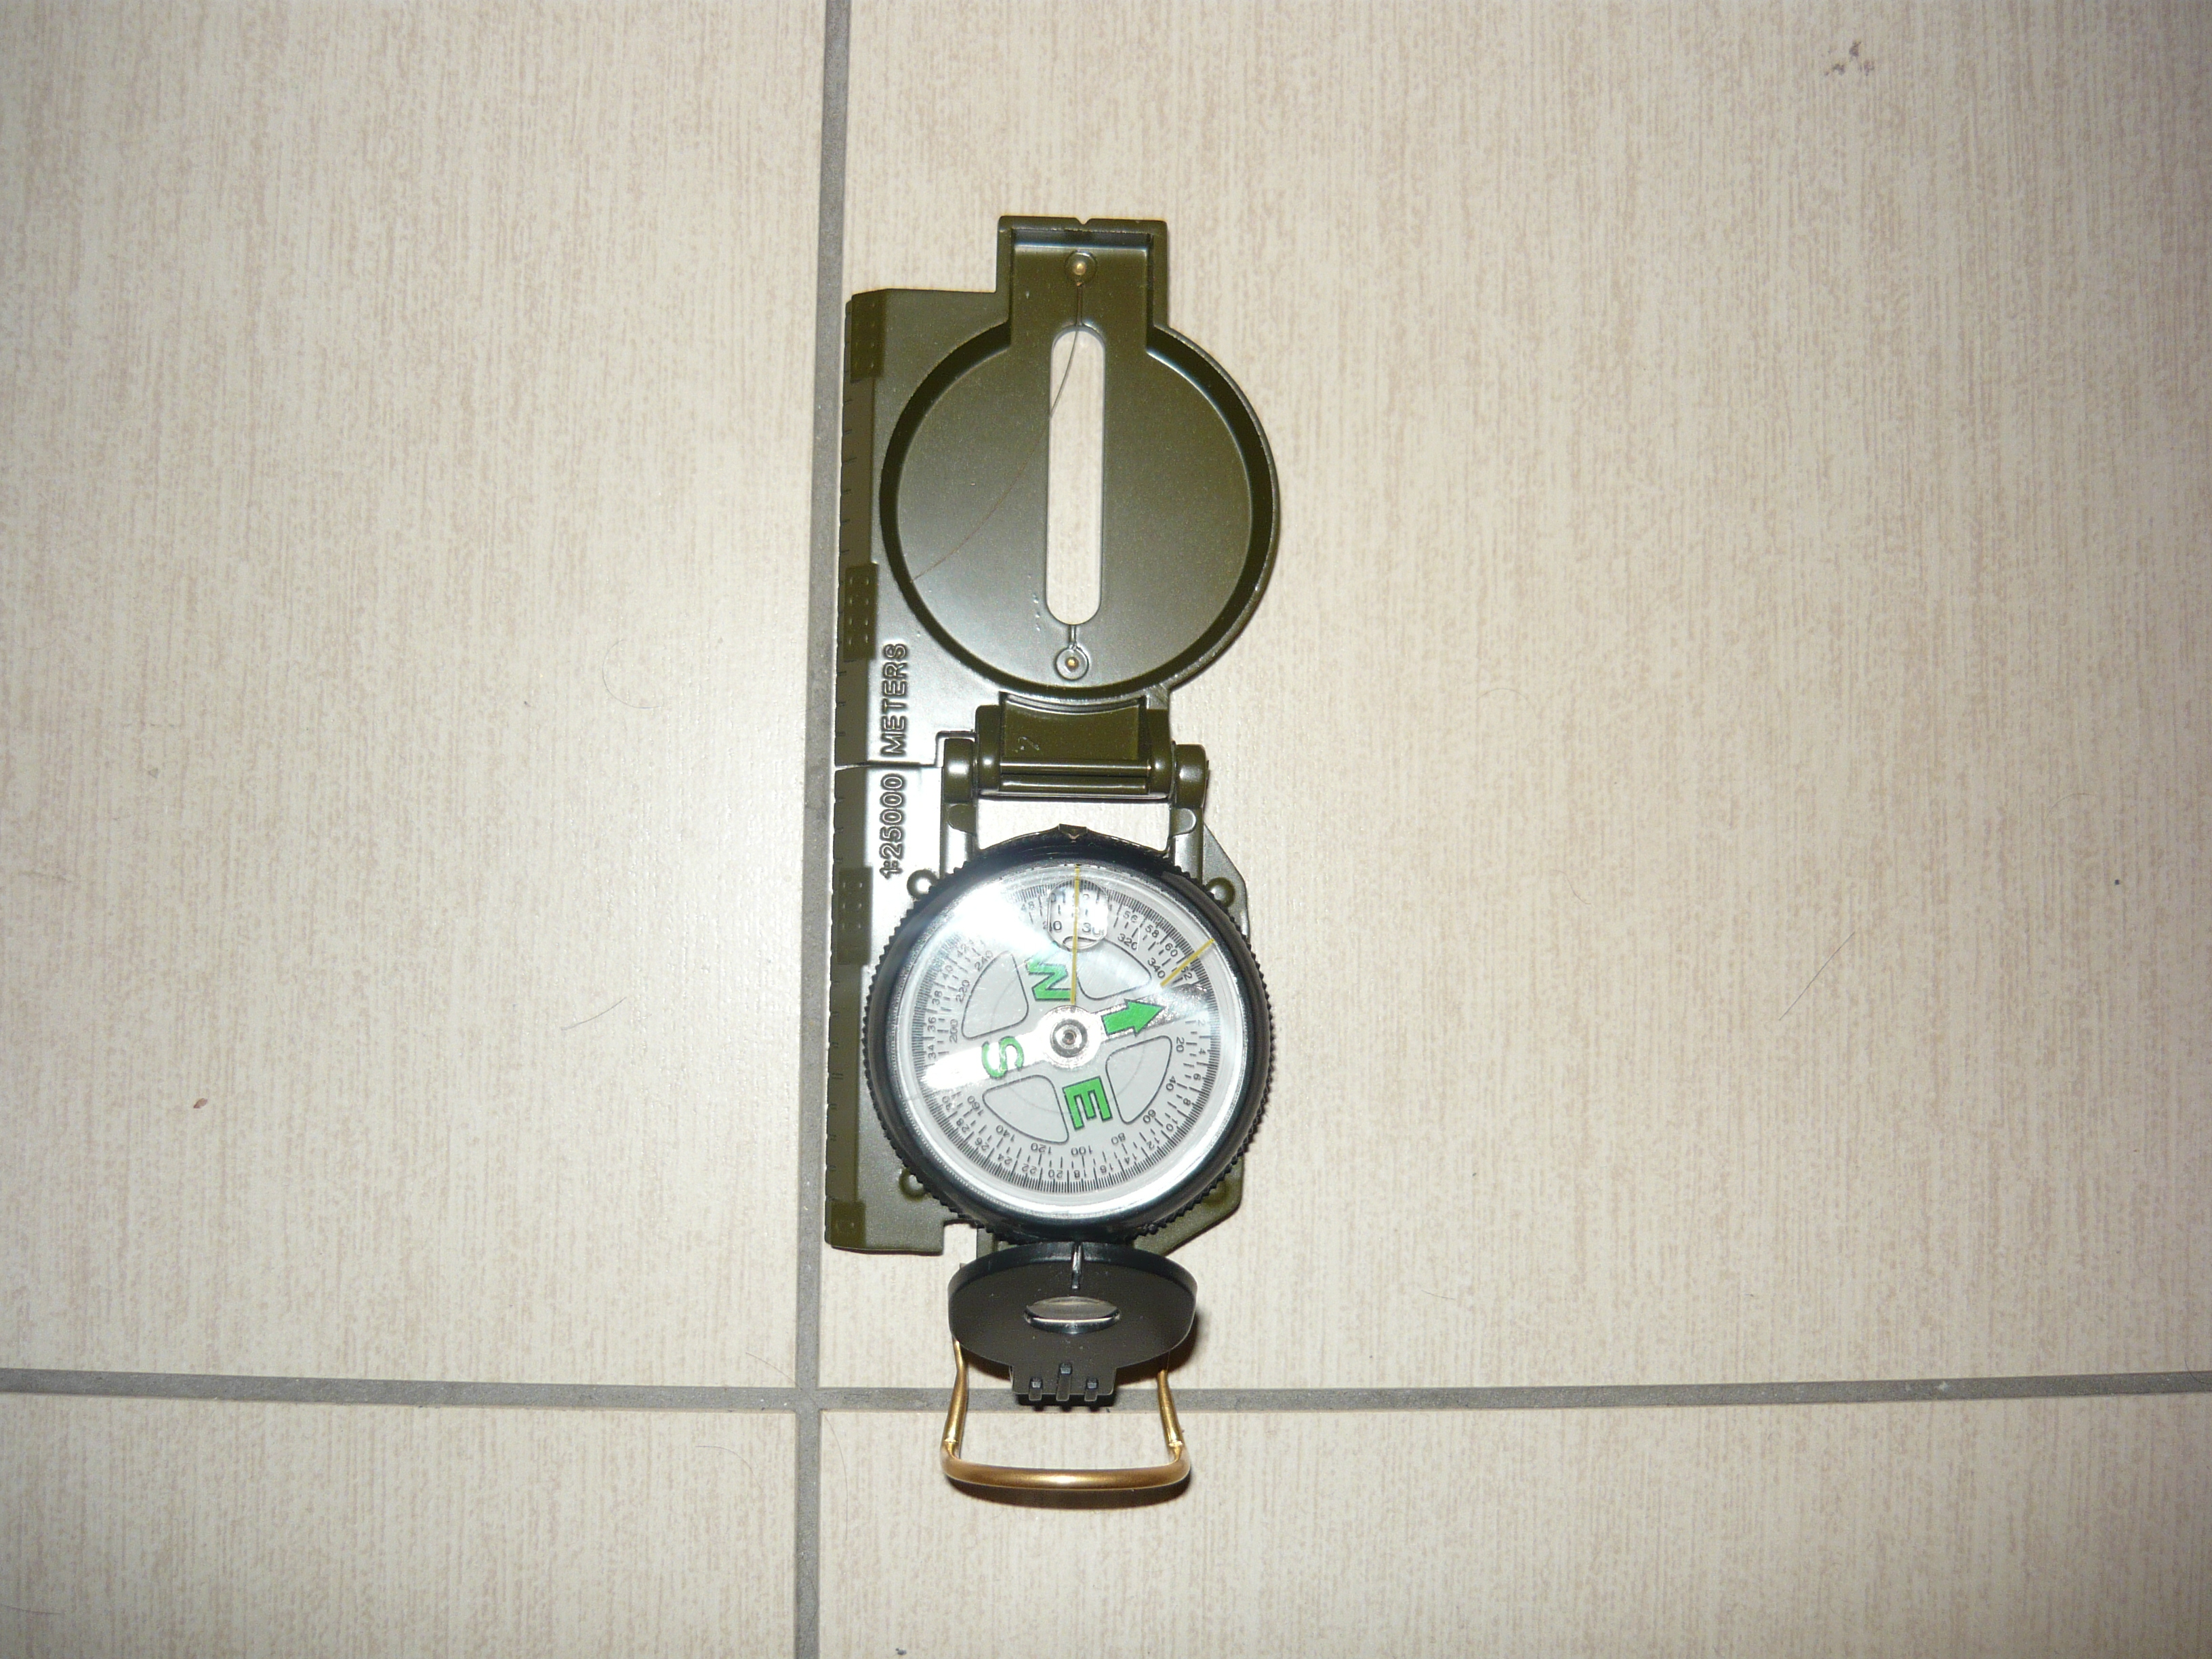
\includegraphics[height=60mm]{../images/ch04/compass02.jpg}
 \caption{Busola przesunięta równolegle o 25 cm,}
 \label{fig:Busola2}
\end{figure}

Niestety wykonane testy pokazały, iż nie jest możliwe wykorzystanie kompasu w celu określenia azymutu robota poruszającego się po podłodze budynku. Jest to spowodowane stosowaniem metalowych prętów zbrojeniowych w stropach budynków, które zakłócają pracę kompasu. Testy zostały wykonane zarówno przy pomocy modułu elektronicznego kompasu jak i tradycyjnej wojskowej busoli. Rysunki \ref{fig:Busola1} oraz \ref{fig:Busola2} przedstawiają odchylenie azymutów wyznaczonych na podłodze budynku. Busola przedstawiona na zdjęciach została przesunięta równolegle o 25 cm w prawo. Wskazywany kierunek północy zmienił się o ponad $90^{\circ}$. Jak widać przy tak dużych wahaniach nie jest możliwe wykorzystanie magnetometru jako elementu jednoznacznie określającego kierunek w którym robot ma się poruszać. Po wielu nieudanych próbach wyeliminowania zakłóceń moduł kompasu został zastąpiony modułem żyroskopu.

% http://www.iemw.tuwien.ac.at/publication/workshop0600/Hauser.html